\documentclass[a4paper,12pt]{article}
\usepackage{a4wide}
\usepackage[pdftex]{hyperref}
\usepackage[german]{babel}
\usepackage[utf8]{inputenc}
\usepackage{amssymb}
\usepackage{csquotes}
\usepackage{wrapfig}
\usepackage{graphicx}
\usepackage{multicol}
\usepackage{amsmath}
\usepackage{enumitem}
\usepackage{polynom}
\usepackage{siunitx}

\setlength{\marginparsep}{1 cm}
\setlength{\topmargin}{-0.6in}
\setlength{\textheight}{9.5in}
\pagestyle{plain}

\polyset{%
   style=C,
   delims={\big(}{\big)},
   div=:
}

% Polynomial long division
\polyset{%
	style=C,
	delims={\big(}{\big)},
	div=:
}

% Differential operator
\newcommand{\diff}[1]{\:\mathrm{d}{#1}}
\newcommand{\pdd}[2]{\frac{\partial #1}{\partial #2}}
\newcommand{\pddn}[3]{\frac{\partial^{#1} #2}{\partial #3^{#1}}}
\newcommand{\dd}[2]{\frac{\mathrm{d}{#1}}{\mathrm{d}{#2}}}
\newcommand{\ddn}[3]{\frac{\mathrm{d}^{#1}{#2}}{\mathrm{d}{#3^{#1}}}}

% N-th root
% \nroot{3}{27}
\newcommand*{\nroot}[2]{\sqrt[\leftroot{-1}\uproot{2}#1]{#2}}
\newcommand*{\ncroot}[4]{\sqrt[\leftroot{#1}\uproot{#2}#3]{#4}}

% 2 component vector
% \tvect{1}{-1}
% \tvec{1}{-1}
\newcommand{\tvect}[2]{%
   \ensuremath{\Bigl(\negthinspace\begin{smallmatrix}#1\\#2\end{smallmatrix}\Bigr)}}
\newcommand{\tvec}[2]{%
    \ensuremath{\left(\negthinspace\begin{matrix}#1\\#2\end{matrix}\right)}}

% 3 component vector
% \rvect{1}{-1}{0}
% \rvec{1}{-1}{0}
\newcommand{\rvect}[3]{%
   \ensuremath{\Bigl(\negthinspace\begin{smallmatrix}#1\\#2\\#3\end{smallmatrix}\Bigr)}}
\newcommand{\rvec}[3]{%
    \ensuremath{\left(\negthinspace\begin{matrix}#1\\#2\\#3\end{matrix}\right)}}

% Long vector arrow
% \xshlongvec{ABC}

% German-style quotation marks %
\MakeOuterQuote{"}

% Number sets
\newcommand{\N}{\mathbb{N}}
\newcommand{\Z}{\mathbb{Z}}
\newcommand{\Q}{\mathbb{Q}}
\newcommand{\R}{\mathbb{R}}
\newcommand{\C}{\mathbb{C}}

\newcommand{\setzero}{\varnothing}

% Mention (small caps)
\newcommand{\mention}[1]{\textsc{#1}}

% Functions
\newcommand{\asin}[0]{\text{asin}}
\newcommand{\acos}[0]{\text{acos}}
\newcommand{\atan}[0]{\text{atan}}
\newcommand{\sgn}[0]{\text{sgn}}
\newcommand{\grad}[0]{\text{grad}}

% Scale
% Usage in math mode: \Scale[1.5]{...equation...} %
\newcommand*{\Scale}[2][4]{\scalebox{#1}{$#2$}}%

% Units
\newcommand{\um}{\text{m}}
\newcommand{\us}{\text{s}}
\newcommand{\ukm}{\text{km}}
\newcommand{\ukg}{\text{kg}}
\newcommand{\uh}{\text{h}}
\newcommand{\ukmh}{\frac{\ukm}{\uh}}
\newcommand{\umpers}{\frac{\um}{\us}}
\newcommand{\umss}{\frac{\ukm}{\us^2}}
\newcommand{\ukgss}{\frac{\ukg}{\us^2}}
\newcommand{\degrees}[1]{\SI{#1}{\degree}}

% Floor / ceil
\newcommand{\floor}[1]{\left\lfloor #1 \right\rfloor}
\newcommand{\ceil}[1]{\left\lceil #1 \right\rceil}

% Circle characters
\newcommand*\circled[1]{
    \tikz[baseline=(char.base)]{
        \node[shape=circle,draw,inner sep=2pt] (char) {#1};
    }
}



\begin{document}

\begin{center}
  {\bf {\large Aufgabenblatt 2 (MI/IT 2020)}}
\end{center}

% Tasks

\begin{enumerate}

\item Wie müssen die Konstanten $A$ und $B$ gewählt werden, damit $f$ überall stetig wird?

$$
  f(x) = \begin{cases}-2\sin(x) & x\in (-\infty,\-\pi/2] \\ A\sin(x)+B & x \in (-\pi/2,\pi/2) \\ \cos(x) & x \in [\pi/2,\infty) \end{cases}
$$

\item $f(x) = \frac{p(x)}{q(x)} = \frac{3x^3+10x^2-x}{x^4-2x^2+1}$. Der Nenner hat die doppelte Nullstelle $1$. Ermitteln Sie die restlichen beiden Nullstellen, indem Sie mittels Polynomdivision den dazugehörigen Linearfaktor abspalten und die entstehende quadratische Gleichung lösen! Führen Sie nun eine Partialbruchzerlegung von $f$ durch! Geben Sie anschließend die Nullstellen und Polstellen von $f$ an!


\item 

\begin{multicols}{2}

In der nebenstehende Skizze ist die Funktion $f(x)$ dargestellt. Es handelt sich um eine skalierte Sinusfunktion. Lesen Sie deren Amplitude sowie Periode ab und geben Sie eine mögliche Funktionsgleichung an!

\columnbreak

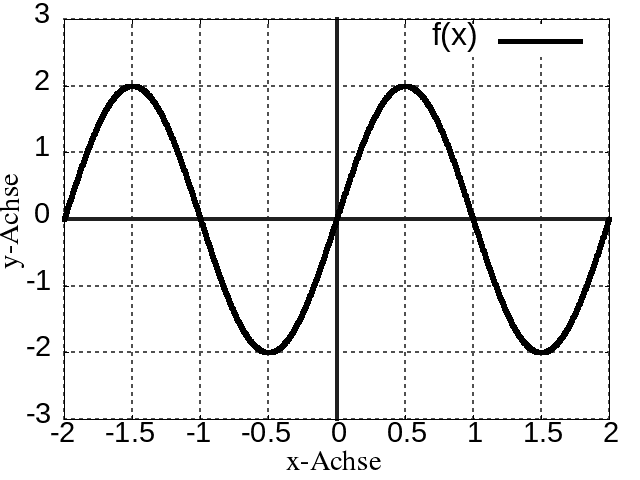
\includegraphics[width=0.35\textwidth]{../pool/ex-graph-read-1-img-a.png}

\end{multicols}




\item Auf welchem der folgenden Intervall hat die Funktion $f(x)=\sin(x)$ (lokale oder globale) Extremwerte? Geben Sie diese gegebenenfalls an! 
$$
	[-\degrees{45},\degrees{45}] \hskip 10pt (-\degrees{45},\degrees{45}) \hskip 10pt (-\degrees{45},\degrees{45}] \hskip 10pt [\degrees{0},\degrees{135})  \hskip 10pt [\degrees{0},\degrees{180}) \hskip 10pt [0,\degrees{180}] \hskip 10pt (225,\degrees{315}) 
$$

\item Der Hyperbelkosinus ist definiert als der symmetrische Anteil der Exponentialfunktion: $\cosh(x) = \frac{e^x+e^{-x}}{2}$. Ist diese Funktion umkehrbar und warum? Wenn nein, gibt es eine Einschränkung des Definitionsbereichs oder Wertebereichs, in der sie umkehrbar ist? Geben Sie gegebenenfalls eine entsprechende Funktionsgleichung an! (Hinweis: Multiplizieren beider Seiten mit $e^x$, Substitution $z=e^x$)

\item Ordnen Sie folgende 12 Funktionen nach Ihrer Wachstumsrate für $x\to\infty$, sodass also für zwei aufeinanderfolgende Funktion $f$ und $g$ in der geordneten Liste gilt $f \in \mathcal{O}(g)$. Entscheiden Sie weiterhin, ob auch $g \in \mathcal{O}(f)$, die Funktionen also gleich stark anwachsen.
(Hinweis: Regel von L'Hôpital)

$$
x^2 \hskip 4mm  3^x \hskip 4mm \ln(x) \hskip 4mm \sqrt{x} \hskip 4mm \hskip 4mm x^{100} \hskip 4mm 10^{100}x \hskip 4mm 2^x \hskip 4mm \ln(\sqrt{x}) \hskip 4mm \ln(x^2) \hskip 4mm (\ln(x))^2 \hskip 4mm x\ln(x) \hskip 4mm x
$$

\item Zeigen Sie anhand der Definition des Hyperbelkosinus (Hyperbelsinus) über die Exponentialfunktion, dass diese Funktion gerade (ungerade) ist!

\end{enumerate}

\newpage

% Solutions

\begin{center}
{\bf {\large Lösungen}}
\end{center}

\begin{enumerate}
	
\item In den einzelnen Abschnitten sind die Teilfunktionen stetig. Untersuchen müssen wir die beiden Übergangsstellen. Wir betrachten zuerst $x=-\pi/2$. Es muss gelten: $\lim\lim\limits_{x\to-\pi/2} f(x) = f(-\pi/2)$. Speziell muss also auch der links und rechtsseitige Grenzwert gleich sein. Es ist

$$
  \lim\limits_{x\to{-\pi/2}^{-}} f(x) = -2\sin(-\pi/2) = 2
$$

und

$$
  \lim\limits_{x\to{-\pi/2}^{+}} f(x) = A\sin(-\pi/2)+ B = -A+B
$$

Analog erhalten wir für die Stelle $x=\pi/2$:

$$
  \lim\limits_{x\to{-\pi/2}^{-}} f(x) = A\sin(\pi/2) + B = A+B
$$

und

$$
  \lim\limits_{x\to{-\pi/2}^{+}} f(x) = \cos(\pi/2) = 0
$$

Durch Gleichsetzen gewinnen wir $2=-A+B$ sowie $A+B=0$. Die Lösung dieses Gleichungssystems lautet $A=-1$ und $B=1$.


\item Nach dem Fundamentalsatz der Algebra wissen wir, dass der Nenner in Linearfaktoren zerlegbar ist:

$$
	x^4-2x^2+1 = (x-1)(x-1)(x-a)(x-b)
$$

Die rechten beiden Faktoren bilden ein Polynom. Dieses ergibt sich zu $\frac{x^4-2x^2+1}{(x-1)(x-1)}$. Da $(x-1)(x-1)=x^2-2x+1$ können wir eine Polynomdivision durchführen:

\[\polylongdiv{x^4-2x^2+1}{x^2-2x+1}\]

Dieses Polynom hat die doppelte Nullstelle $a=b=-1$. Wir können für die Partialbruchzerlegung ansetzen:

$$
	\frac{3x^3+10x^2-x}{(x-1)^2(x+1)^2} = \frac{A}{x-1} + \frac{B}{(x-1)^2} + \frac{C}{x+1} + \frac{D}{(x+1)^2}
$$

Wir bringen zuerst alle Brüche auf einen gemeinsamen Nenner

\begin{alignat*}{3}
	\frac{A}{x-1}     \cdot && \frac{(x-1)(x+1)^2}{(x-1)(x+1)^2} &= \frac{Ax^3+Ax^2-Ax-A}{(x-1)^2(x+1)^2} \\
	\frac{B}{(x-1)^2} \cdot && \frac{(x+1)^2}{(x+1)^2}           &= \frac{Bx^2+2Bx+B}{(x-1)^2(x+1)^2} \\
	\frac{C}{x+1}     \cdot && \frac{(x+1)(x-1)^2}{(x+1)(x-1)^2} &= \frac{Cx^3-Cx^2-Cx+C}{(x-1)^2(x+1)^2} \\
	\frac{D}{(x+1)^2} \cdot && \frac{(x-1)^2}{(x-1)^2}           &= \frac{Dx^2-2Dx+D}{(x-1)^2(x+1)^2} 
\end{alignat*}

Zusammenfassen nach gleichen Potenzen liefert:

$$
	\frac{(A+C)x^3+(A+B-C+D)x^2+(-A+2B-C-2D)x+(-A+B+C+D)}{(x-1)^2(x+1)^2}
$$

Durch Koeffizientenvergleich mit $\frac{3x^3+10x^2-x}{(x-1)^2(x+1)^2}$ erhalten wir

\begin{alignat*}{7}
	3  &= A  &   &    & + & C &   &    \\
	10 &= A  & + &  B & - & C & + &  D \\
	-1 &= -A & + & 2B & - & C & - & 2D \\
	0  &= -A & + &  B & + & C & + &  D
\end{alignat*}

Dieses lineare Gleichungssystem kann etwa mit dem Gauß-Algorithmus oder dem Basisaustauschverfahren gelöst werden und hat die Lösung $A=4$, $B=3$, $C=-1$ und $D=2$.

Damit lautet die Partialbruchzerlegung:

$$
	\frac{3x^3+10x^2-x}{(x-1)^2(x+1)^2} = \frac{4}{x-1} + \frac{3}{(x-1)^2} - \frac{1}{x+1} + \frac{2}{(x+1)^2}
$$

Die Nullstellen von $f$ erhält man durch Gleichsetzen des Zählers $3x^3+10x^2-x$ mit $0$. Da kein konstantes Glied vorkommt, ist $x_1=0$ eine Nullstelle und es verbleibt, die quadratische Gleichung $3x^2+10x-1=0$ zu lösen. Diese hat die Lösungen

$$
	x_{2,3} = -\frac{5}{3} \pm \sqrt{\frac{25}{9}+\frac{3}{9}} = -\frac{5}{3} \pm \frac{1}{3}\sqrt{28} = = -\frac{5}{3} \pm \frac{2}{3}\sqrt{7}
$$

Die Nullstellen des Nenner sind verschieden von den Nullstellen des Nenners. Somit hat $f$ die zwei (doppelten) Polstellen $-1$ und $1$ sowie die drei Nullstellen $0$ und $-\frac{5}{3} \pm \frac{2}{3}\sqrt{7}$.


\item Die Amplitude ist der Ausschlag bezogen auf die Nulllage und beträgt $2$. Manchmal wird unter Amplitude auch die Differenz zwischen dem größten und dem kleinsten Funktionswert (hier 4) verstanden. Die Periode beträgt $2$. Aus diesen Angaben folgt für die Funktionsgleichung $f(x) = 2\cdot\sin(\pi x)$. 



\item 

\begin{enumerate}
	\item $[-\degrees{45},\degrees{45}]$ Globales Minimum bei $-\degrees{45}$. Globales Maximum bei $\degrees{45}$.
	\item $(-\degrees{45},\degrees{45})$ Keine Extremwerte.
	\item $(-\degrees{45},\degrees{45}]$ Globales Maximum bei $\degrees{45}$.
	\item $[\degrees{0},\degrees{135})$ Globales Minimum bei $\degrees{0}$. Globales Maximum bei $\degrees{90}$.
	\item $[\degrees{0},\degrees{180})$ Globale Minimum bei $\degrees{0}$. Globales Maximum bei $\degrees{90}$.
	\item $[\degrees{0},\degrees{180}]$ Globale Minimum bei $\degrees{0}$ und $\degrees{180}$. Globales Maximum bei $\degrees{90}$.
	\item $(225,\degrees{315})$ Globales Minimum bei $\degrees{270}$
\end{enumerate}


\item Da $\cosh$ per Definition symmetrisch ist, gilt z.B. $\cosh(1) = \cosh(-1)$. Damit ist aber die Injektivität verletzt, da ein Funktionswert doppelt angenommen wird. Schränken wir den Definitionsbereich auf die nichtnegativen Zahlen ein, ist $\cosh$ streng monoton steigend, denn für $x>y>0$ gilt:

\begin{alignat*}{1}
	\implies x &> y \\
	\implies e^x &> e^y \text{ da Exponentialfunktion streng monoton steigend} \\
	\implies e^x (1-e^{-x-y}) &> e^y (1-e^{-x-y}) \\
	\implies e^x-e^{-y} &> e^y - e^{-x} \\
	\implies e^x + e^{-x} &> e^y + e^{-y} \\
	\implies \cosh(x) &> \cosh(y)
\end{alignat*}

Der Übergang von der zweiten zur dritten Zeile ist korrekt, das Vorzeichen dreht sich nicht um, da $-x-y<0$ und damit $e^{-x-y} < 1$ , also $1-e^{-x-y} > 0$ ist.

Der minimale Wert für $\cosh(x)$ im Intervall $[0, \infty)$ muss aufgrund der steigenden Monotonie bei $x=0$ liegen, hier ist der Funktionswert $\cosh(0) = \frac{e^0+e^0}{2} = 1$. Schränken wir daher noch den Funktionsbereich auf $[1, \infty]$, werden alle Funktionswerte angenommen und die Surjektivität ist erfüllt.

Zusammengefasst: $\cosh$ ist für $x \in [0, \infty)$ und $y \in [1,\infty]$ injektiv und surjektiv und damit umkehrbar.

Die Umkehrfunktion finden wir durch Umstellen:

\begin{alignat*}{1}
	\frac{e^x+e^{-x}}{2} &= y \\
	 e^x+e^{-x} &= 2y \\
	 e^x \cdot e^x + e^{-x} e^x &= 2ye^x \\
	 (e^x)^2 - 2ye^x + 1 &= 0 \\
	 e^x &= y \pm \sqrt{y^2-1} \\
\end{alignat*}

Jetzt ist die Frage, welche dieser beiden Lösungen die richtige ist.

Es ist $y^2-1 < y^2$ und damit $\sqrt{y^2-1} < \sqrt{y^2}$. Für $y \in [1,\infty]$ gilt damit besonders $\sqrt{y^2-1} < y$, also ist $y - \sqrt{y^2-1} > 0$. Weiterhin muss $x$ im Intervall $x \in [0, \infty)$ liegen. Das ist aber nur für die zweite Lösung mit $y+\dots$ möglich, für $y \ge 1$ gilt $y - \sqrt{y^2-1} \le 1$ (siehe unten). Dann wäre aber $e^x \le 1$ und $y\le 0$, was nicht im erlaubten Intervall für $y$ liegt.

\begin{alignat*}{2}
              & y - \sqrt{y^2-1} \le  1 \\
	\iff & y-1  \le   \sqrt{y^2-1} \\
	\iff & (y-1)^2  \le   y^2-1 \\
	\iff & y^2-2y+1  \le   y^2-1 \\
	\iff & -2y  \le   -2 \\
	\iff & 2y  \ge   2 \\
	\iff & y  \ge   1 \\
\end{alignat*}

Somit erhalten wir für die Umkehrfunktion:

$$
	\cosh^{-1}(y) = \ln(y + \sqrt{y^2-1})
$$

\item Zur Erinnerung: $f \in \mathcal{O}(g)$ bedeutet, dass der Quotient $\frac{f(x)}{g(x)}$ für große $x$ endlich bleibt, also der Grenzwert $x\to\infty$ existiert.

Die geordnete Liste lautet:

$$
  \ln(\sqrt{x}) \simeq \ln(x) \simeq \ln(x^2) \prec (\ln(x))^2 \prec \sqrt{x} \prec x \simeq 10^{100}x  \prec x\ln(x)  \prec x^2 \prec x^{100} \prec 2^x \prec 3^x
$$

Dabei bedeutet $f \prec g$, dass $f$ langsamer wächst als $g$ ($g \notin \mathcal{O}(f)$); während $f \simeq g$ bedeutet, dass beide Funktionen ähnlich schnell wachsen ($g \in \mathcal{O}(f)$).

Zum Beweis (im Folgenden ist immmer der Grenzwert $x \to \infty$ gemeint)

\begin{itemize}
	\item Wegen $\ln(\sqrt{x}) = \frac{1}{2}$ und $\ln(x^2)=2\ln(x)$ unterscheiden sich die ersten drei Funktionen nur um einen Vorfaktor, ihr Quotient ist also konstant.
	\item $\frac{\ln(x)}{\ln(x)\ln(x)} = \frac{1}{\ln(x)}$ konvergiert gegen $0$.
	\item Regel von L'Hôpital: $\lim \frac{\ln(x)^2}{x^{1/2}} = \lim \frac{2\ln(x)\frac{1}{x}}{\frac{1}{2}x^{-1/2}} = 4 \lim \frac{\ln(x)}{x^{1/2}}$. Erneut Regel von L'Hôpital: $\lim \frac{\ln(x)}{x^{1/2}} = \lim \frac{1/x}{\frac{1}{2} x^{-1/2}} = 2 \lim \frac{1}{\sqrt{x}} = 0$
	\item $\frac{\sqrt{x}}{x} = \frac{1}{\sqrt{x}}$ konvergiert gegen $0$.
	\item Alle linearen Funktion $c*x$ für $c\in\R\lbrace0\rbrace$ unterscheiden sich nur um einen konstanten Vorfaktor, ihre Quotienten sind konstant.
	\item $\frac{x}{x\ln(x)} = \frac{1}{\ln(x)}$ konvergiert gegen $0$.
	\item $\frac{x\ln(x)}{x^2} = \frac{\ln(x)}{x}$. Regel von L'Hôpital: $\lim \frac{\ln(x)}{x} = \lim \frac{1/x}{1} = 0$
	\item $\frac{x^2}{x^{100}} = \frac{1}{x^{98}}$ konvergiert gegen $0$.
	\item Für $\lim \frac{x^{100}}{2^x}$ liefert die Regel von L'Hôpital $\frac{100}{\ln(2)} \lim \frac{x^{99}}{2^x}$. Setzt man die Anwendung der Regel von L'Hôpital fort, erhält man schließlich $\frac{100!}{\ln(2)^{100}} \lim \frac{1}{2^x} = 0$.
	\item $\lim \frac{2^x}{3^x} = \lim \left(\frac{2}{3}\right)^x = 0$ (geometrische Folge).
\end{itemize}


\item Zur Erinnerung: Eine Funktion $f$ heißt gerade, wenn $f(x) =f(-x)$ gilt und ungerade, wenn $f(x) = -f(-x)$ gilt.

\begin{itemize}
	\item $2 \cosh(x) = e^x+e^{-x} =   e^{(-x)} + e^{-(-x)}  = 2  \cosh(-x)$
	\item $2 \sinh(x) = e^x-e^{-x} = -(e^{(-x)} - e^{-(-x)}) = - 2 \sinh(-x)$
\end{itemize}

\end{enumerate}

\end{document}

